\documentclass[thesis.tex]{subfiles}

\begin{document}

\chapter{Evaluation}\label{chap:eva}

This chapter contains the results of the experiments from the different strategies and methods as discussed in \autoref{chap:main}. The experiment shall show if the postulated SpeedCam approach achieves the goals (\autoref{sec:intro:goals}). At first, it describes the test environment so that the experiment is repeatable and the results are verifiable. Then it list the different experiment configuration and lastly their results, which will be interpreted and discussed. The following \autoref{chap:concl} draws the conclusion of these results.

\section{Test environment}

There are two different used test environments to validate the theses.
The first one is a local virtual machine of Ubuntu 16.04 LTS under a Windows 10 host. The host is an i7-6700K with 16GB DDR-2133. The image is placed on a SSD 850 EVO. The virtual machine can use 4GB of RAM and 4 logical cores. Inside this VM is a virtual network running the default topology as shown in \autoref{fig:eva:defaultTopo}. The installation process is the same as described in the SCION readme.me\footnote{\url{https://github.com/scionproto/scion/blob/master/README.md}, 07.04.2018}. Each component of the virtual network is running as a own process and interact with each other.

\begin{figure}
	\centering
	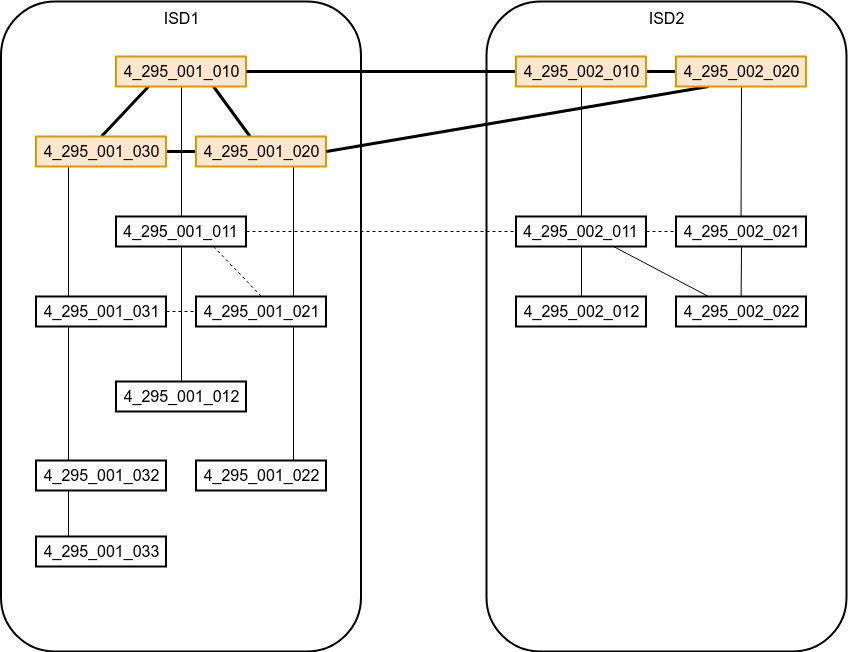
\includegraphics[height=8cm]{default_topo}
	\caption*{\tiny{\url{https://github.com/scionproto/scion/blob/master/doc/fig/default_topo.png}, 07.04.2018}}
	\caption{Default topology}
	\label{fig:eva:defaultTopo}
\end{figure}

The second environment is that of SCIONLab in its current state. A part of this network is seen in \autoref{fig:eva:scionLabTopo}, which is the topology after a few exploration episodes. It does not represent the complete topology, only the current observed one. The inspector program is running on the same machine as the SCPB, while the scripts for information about border router interfaces and path server requests are running on different machines. The inspectors machine is a virtual machine \todo{Specs dieser virtuellen maschine erfragen}. One major problem with that test environment was that there weren't border router information for all nodes in the network. This results in fewer usable nodes than there were ASes as seen in \todo{Liniendiagram mit exlporierten und nutzbaren ASes anzeigen}, which results in a lower precision. This has to be considered in the interpretation of the results.

\begin{figure}
	\centering
	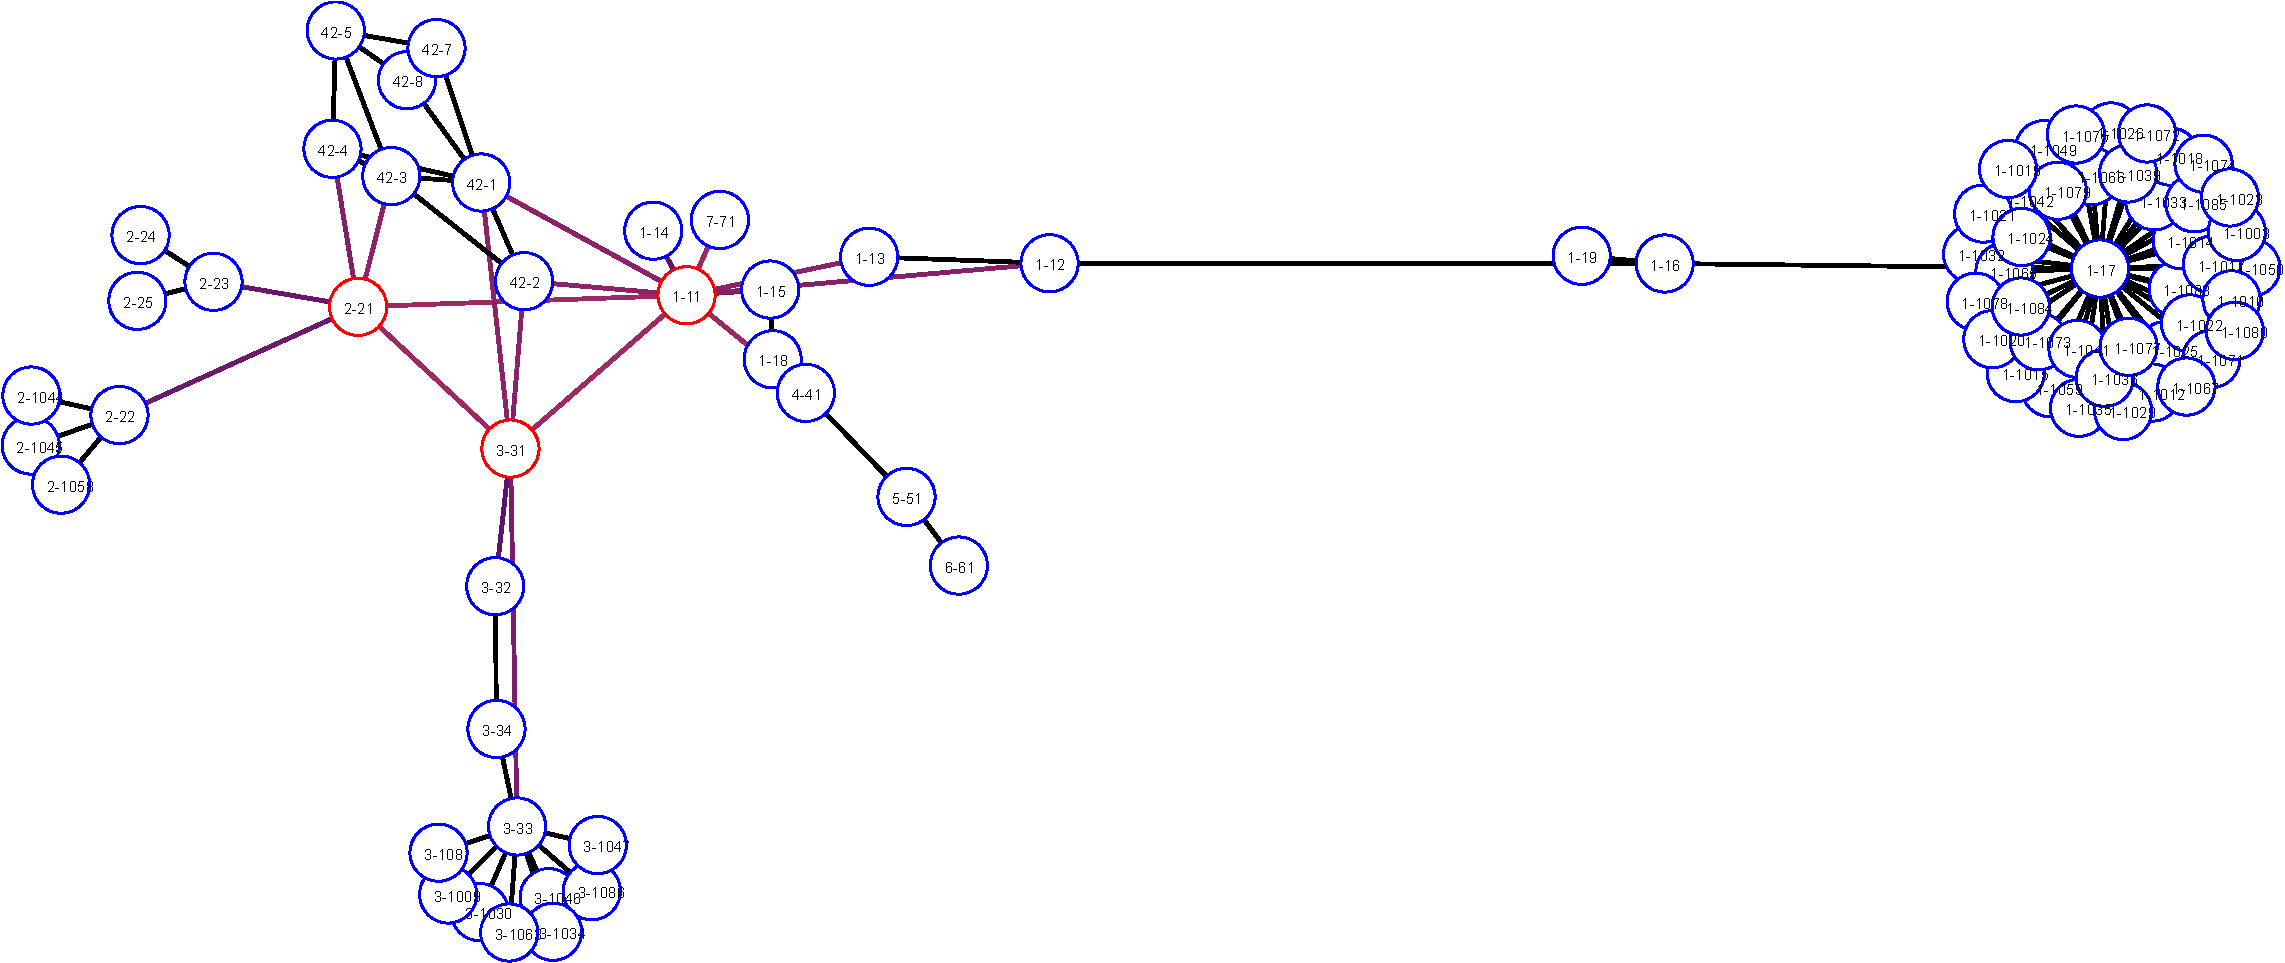
\includegraphics[width=.9\linewidth]{scionLabTopology.pdf}
	\caption{Part of SCIONLab topology}
	\label{fig:eva:scionLabTopo}
\end{figure}

\section{Experiment}

The experiment was ran on the SCIONLab network over 48 hours and ran multiple configurations of the SpeedCam program simultaneously. These can be found in the appendix \todo{Das Script im appenndix hinzufügen} and differ from the standard configuration in its each instance, which are described here:

\begin{easylist}
	# \textit{Standard} using the default values for the program. All weights are equal to one, the interval is a fixed to 10 seconds and it uses 20\% of the network nodes. They were set intuitively while developing the software and serve as a baseline. This configuration used a history of six episodes for each node.
	# \textit{Const} uses only one node as a SpeedCam and does not scale with the network. This shall show the inefficiency of such strategy for dynamic, unexplored networks like SCIONLab.
	# \textit{Linear01} uses 10\%, \textit{Linear033} 30\% of the network nodes and will be used the evaluate the different scale methods.
	# \textit{Log} uses a logarithmic scale with the base of 10 to calculate the amount of SpeedCams. As already discusses it is expected to result in a lower precision than the linear scaling methods.
	# \textit{Random} waits a random amount of time between ten seconds to one hour between the inspections, while \textit{Fixed} starts an inspection every minute. 
	# \textit{Experience} uses the strategy by using past inspection to predict the next one. \textit{Experience12} uses twice as much episodes (total of 12) and \textit{Experience03} uses half as much with a total of only 3 episodes. The experience strategy starts with the random strategy until there are 5 data points.		
\end{easylist}

Each instance writes the result of an inspection to a .JSON file containing the complete network graph with past episodes and also the result of the inspection run. 

A Prometheus server is additionally running to provide a baseline of the measured traffic inside the network. This instance fetch data from all border router in an interval of 15 seconds. The difference to the inspector is, that the Prometheus server fetches always the metrics. The data will be used to calculate the precision of the monitored data with \autoref{equo:qualitySelection}, where $\text{traffic}(N)$ is equals to the Prometheus server data. 

Because of the missing or irregular set capacity information a congestion could not be detected, but can only be guessed. This results in unverifiable cases of \autoref{tab:classifyUser}. Instead the hit rate of finding maximums is used to calculate the quality of a configuration. The inspector and the Prometheus server will sort the monitored ASes by their bandwidth for a given timespan. When the position of the inspectors highest ASes only differs by a maximum of 3 from the servers, it will considered as a hit. Otherwise, the inspector guessed the wrong AS and this will be considered as a miss. 

The performance influence of the inspector is measured with the UNIX tool \textit{top} and creates a snapshot of the memory and CPU usage of the programs every 5 seconds. It was build with Go 1.9.5 linux/amd64 without any additional flags.

\section{Result}
This part will list the results of the previously described configuration.

\subsection{Hit and miss rate}

\todo{Stacked bar chart for each diagram}

\subsection{Precision}

\todo{Liniendiagram über zeit mit Prometheus data und den inspector daten}

\subsection{Performance}

The performance impact of SpeedCam on the system is minimal as seen in \autoref{fig:eva:performance}. Without the outliers, no configuration uses more than 1\% of the CPUs computation time and uses in average fewer than 0.5\%. The main impact of the CPU is the amount of utilized SpeedCams as seen in the linear configuration. The more SpeedCams existing, the more candidate scores needs to be calculated and the more monitoring results needs to get parsed. The random and the experience based configuration uses the fewest CPU in average, because most of the time they are sleeping and do not utilize the CPU.

The memory impact has a similar image as seen in \autoref{fig:eva:performance:mem}. No configuration needed more than 1.5\% of the memory. The amount of episodes per node has little to zero influence of the memory as seen for the experience configuration. A higher influence is the amount of used SpeedCams as seen for the \textit{const} configuration with always 1 SpeedCam, which uses nearly constant 1.1\% of the memory.

All in all does have no configuration a significant impact on the systems performance for the SCIONLab network. The goal was to use 5\% or fewer resources, which was achieved.
\begin{figure}
	\centering
	\begin{subfigure}{.95\linewidth}
		\centering
		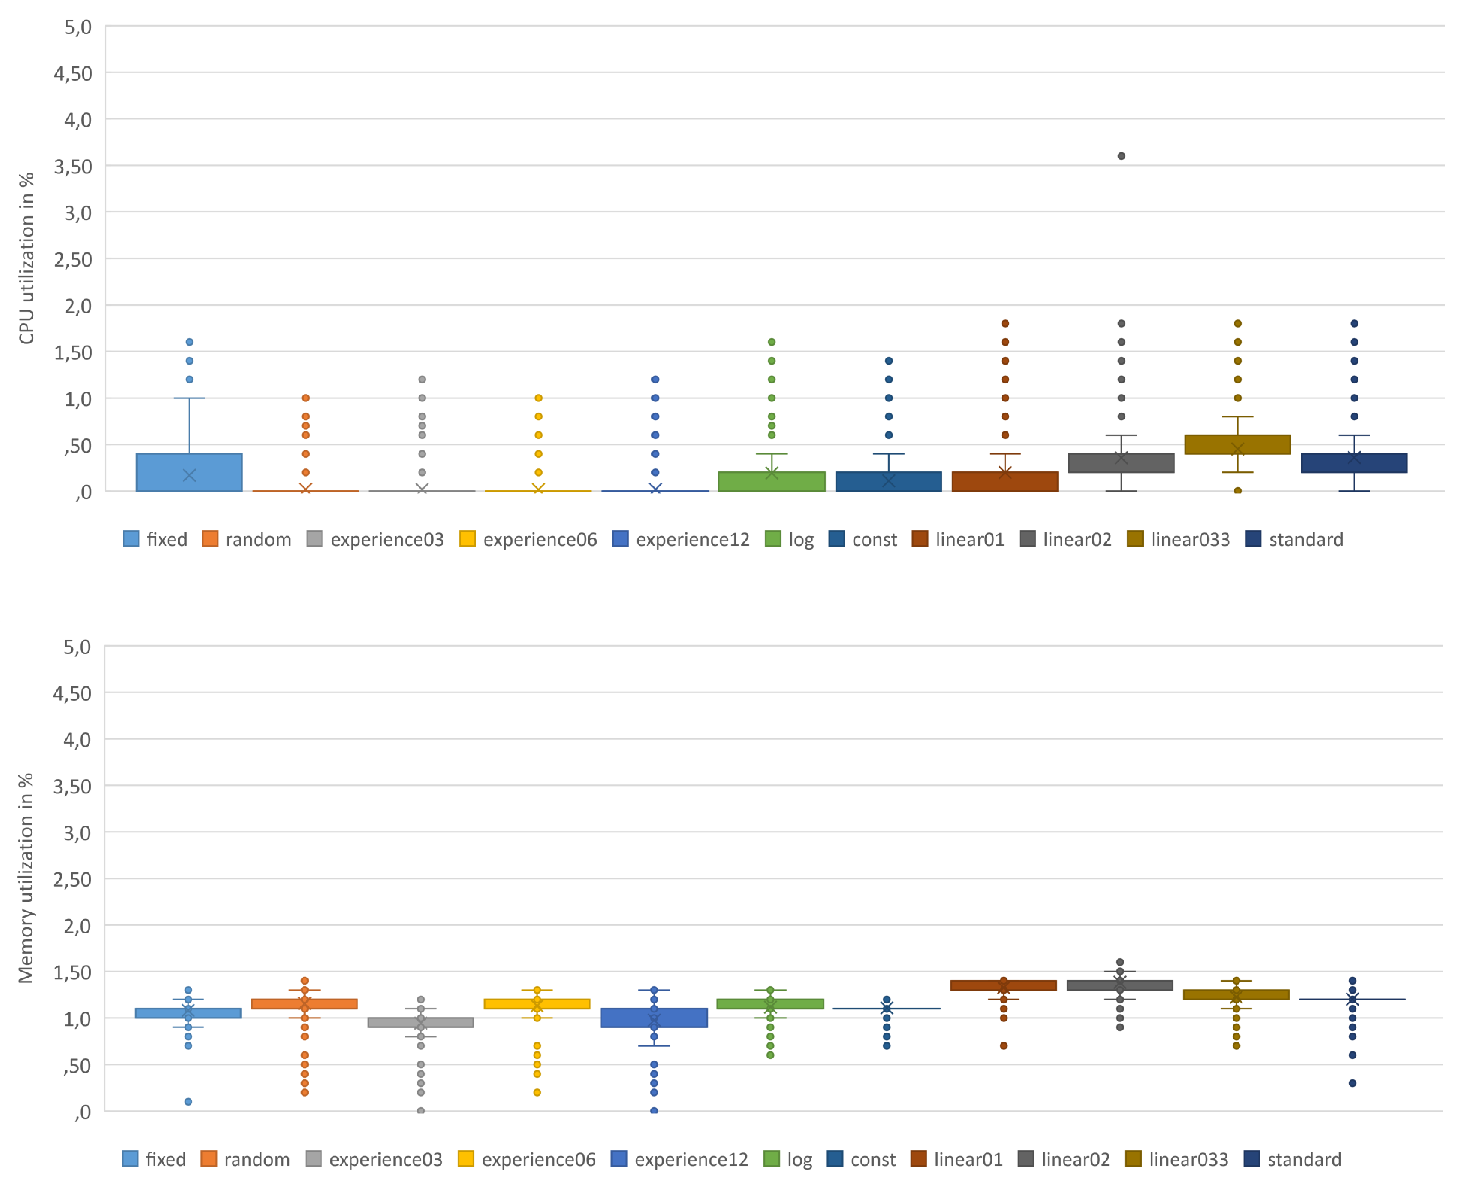
\includegraphics[trim={0mm 100mm 0mm 0mm},clip,width=0.98\textwidth]{performance_diagrams.pdf}
		\caption{CPU usage in \%}
		\label{fig:eva:performance:cpu}
	\end{subfigure}
\hfill
	\begin{subfigure}{0.95\linewidth}
		\centering
		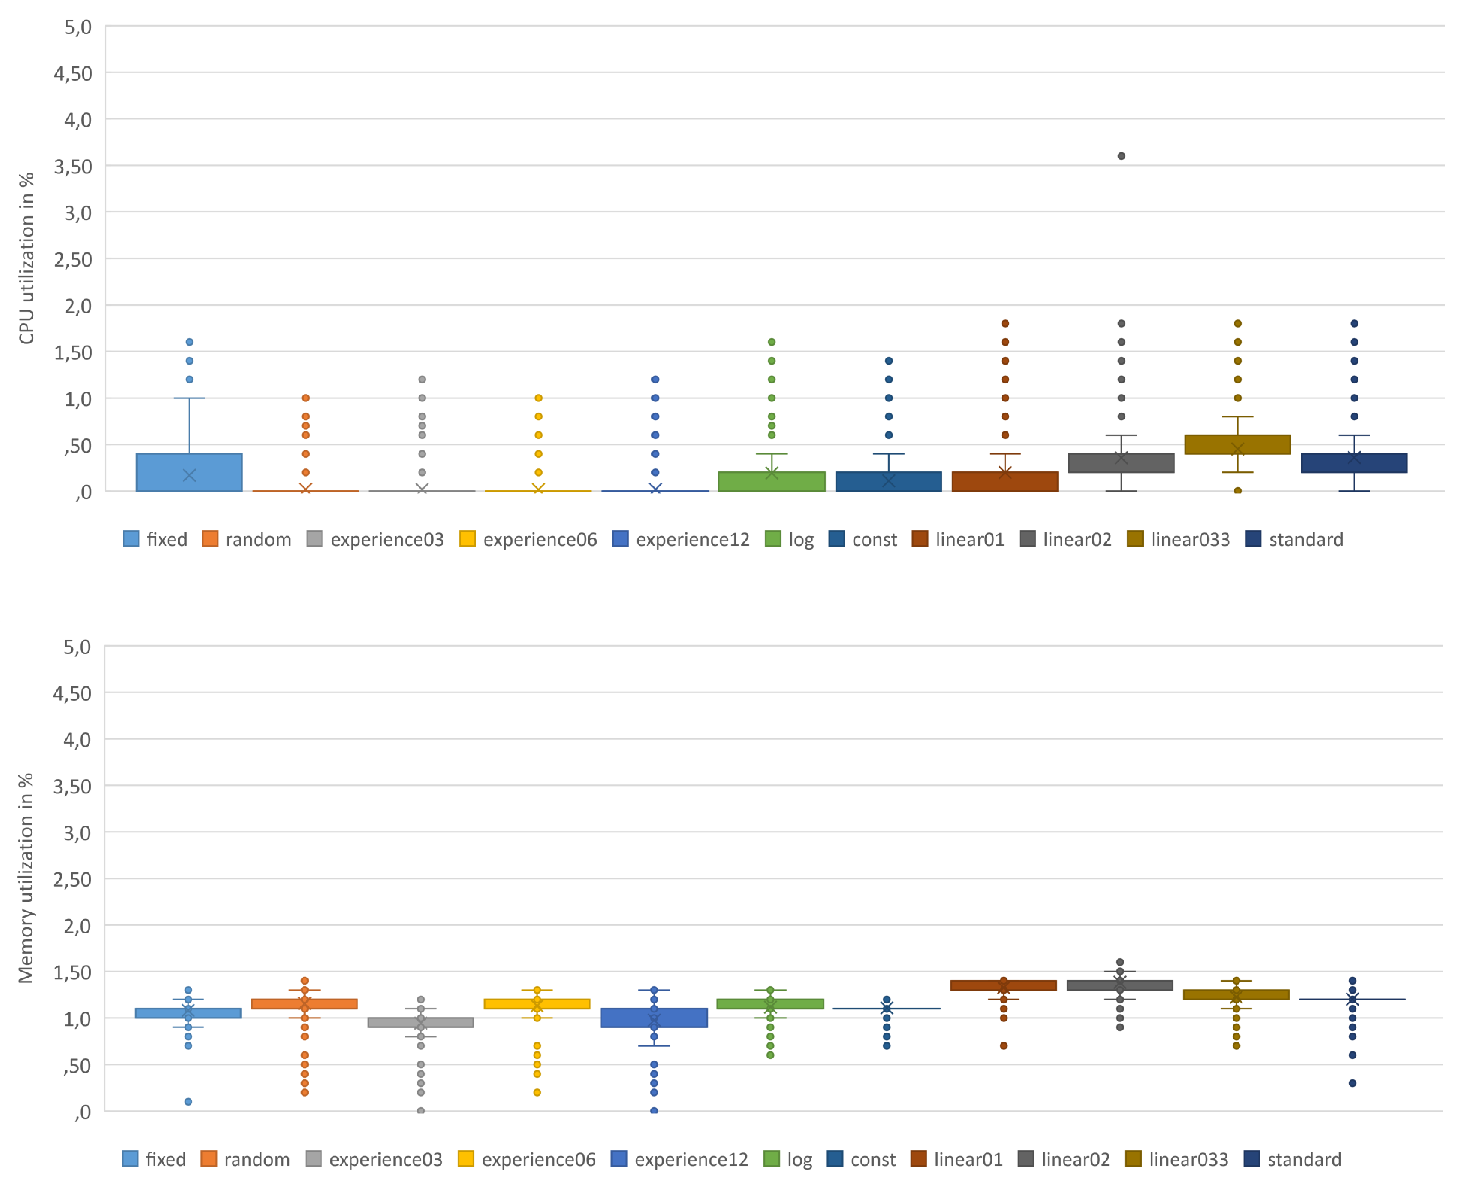
\includegraphics[trim={0mm 0mm 0mm 100mm},clip,width=0.98\textwidth]{performance_diagrams.pdf}
		\caption{Memory usage in \%}
		\label{fig:eva:performance:mem}
	\end{subfigure}
	\caption{Performance impact off configuration over 48h}
	\label{fig:eva:performance}
\end{figure}

\todo{Network traffic wegen SpeedCam über die Zeit anzeigen}

\subfilebib % Makes bibliography available when compiling as subfile
\end{document}